\begin{sitedescription}{CDS}

\begin{center}
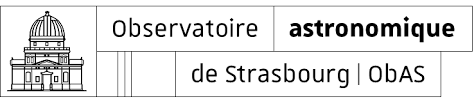
\includegraphics[height=3cm]{Participants/Logos/OAS.png}
\end{center}

The Observatoire Astronomique de Strasbourg (ObAS) is a Joint Research Unit
(UMR7550) of the CNRS and of the Université de Strasbourg. ObAS hosts the 
Centre de Données astronomiques de Strasbourg (Strasbourg astronomical Data 
Centre CDS, http://cds.unistra.fr). Since its creation in 1972, the CDS has 
been providing reference services which are widely used by the world-wide 
astronomical community with more than 1 million queries/day on average in 
2017. The CDS is labelled as a Research Infrastructure in the French national
Research Infrastructure Roadmap. Since 2006 CDS has been the coordinator,
on behalf of the CNRS, of all the projects funded by the European Commission
to support the implementation of European Virtual Observatory. 

% PIC:
% see: http://ec.europa.eu/research/participants/portal/desktop/en/organisations/
%
% See ../proposal.tex, section Members of the Consortium for a
% complete description of what should go there

\subsubsection*{Curriculum vitae}

% Curriculum of the personnel at this institution. This includes
% to-be-hired people for which there is a tentative candidate.

%\input{CVs/First.Last.tex}
%\input{CVs/First.Last.tex}

\input{CVs/Mark.Allen.tex}
\input{CVs/Thomas.Boch.tex}
\input{CVs/Sebastien.Derriere.tex}

\begin{participant}[type=R,PM=12,salary=4200]{Software Engineer}
    We intend to hire a software engineer for 12 months during the project to be be supervised at CDS to work on developments defined in Task \taskref{applications}{astro}. We aim to hire someone in the period of months 12-24. 
\end{participant}

% For other to-be-hired person, please include here something like:
% \begin{participant}[type=res,PM=3,salary=5900]{NN}
%  <a _short_ description of the qualifications of whom you want to hire>
% \end{participant}

\subsubsection*{Publications, products, achievements}

\begin{compactenum}
  \item F. Genova, M. G. Allen, C. Arviset, A. Lawrence, F. Pasian, E. Solano, J. Wambsganss, Euro-VO - Coordination of Virtual Observatory activities in Europe, Astronomy and Computing, 2015, Volume 11, p. 181-189
  \item F. Genova et. al 2017, Building a Disciplinary, World-Wide Data Infrastructure. Data Science Journal, 16: 16, pp. 1-13, DOI: https://doi.org/10.5334/dsj-2017-016
  \item P. Fernique, M. G Allen, T. Boch, A. Oberto, F-X. Pineau, D. Durand, C. Bot, L. Cambresy, S. Derriere, F. Bonnarel, F. Genova, Hierarchical Progressive Surveys - Multi-resolution HEALPix data structures for astronomical images, catalogues and 3-dimensional data cubes.  2015, A \& A, 578, A114 
  \item M. Baumann, T.Boch, New Python developments to access CDS services, Proceedings of The Astronomical Data Analysis Software and Systems conference 2018.
\end{compactenum}

\subsubsection*{Relevant projects or activities}

\begin{compactenum}
  \item ESCAPE (EC funded project, 2019-2023, \#824064, INFRAEOSC-0402018)
  \item ASTERICS (EC funded project, 2015-2019, \#653477, Research and Innovation Action)
  \item AENEAS (EC funded project,  2017-2020, \#731016, Research and Innovation Action)
  \item CoSADIE - Collaborative and Sustainable Astronomical Data Infrastructure for Europe (EC funded project \#312559, 2012-2015, CSA)
  \item RDA Europe - the European plug-in to the Research Data Alliance (RDA) (EC funded project \#632756, 2014-2016, CSA)
\end{compactenum}

\subsubsection*{Significant infrastructure}

CDS is data centre for reference astronomy data. CDS runs physical infrastructure for 1Petabyte. Connected to French national network RENATER. Computing power for X-Match and generation of all-sky survey data. Currently running prototype notebook servers.


\end{sitedescription}
%%% Local Variables:
%%% mode: latex
%%% TeX-master: "../pro%%% End:
